\chapter{Application Design}

\section{ERDs}
\subsection{Initial ERD}
\begin{figure}[ht]
    \centering
    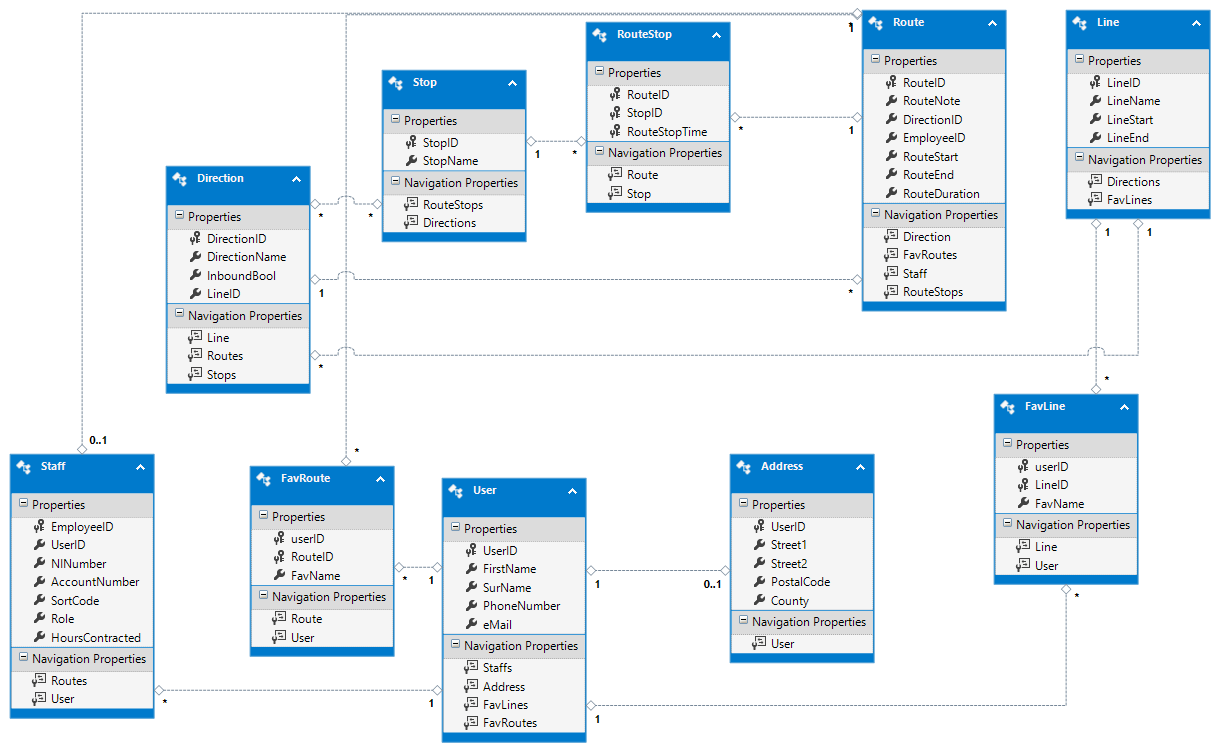
\includegraphics[width=\linewidth]{EntityDesignerDiagram}
    \caption{Initial ERD, corresponding to what we thought the database would look like}
  \end{figure}

\subsection{Final ERD}
\begin{figure}[ht]
    \centering
    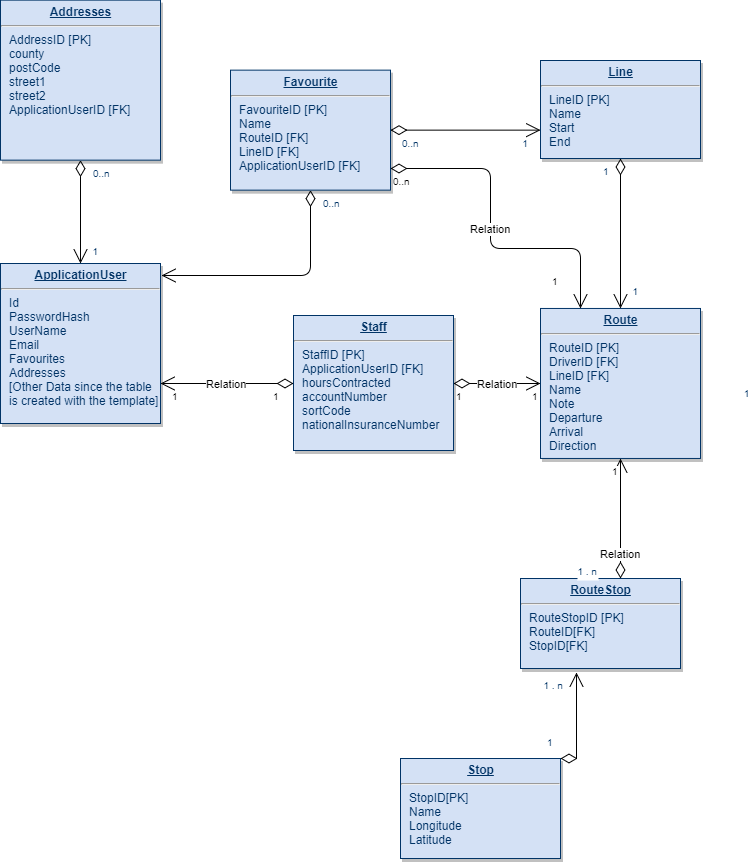
\includegraphics[width=\linewidth]{FinalERD}
    \caption{Final ERD, obtained whilst making the Models and creating the database}
  \end{figure}

In order to obtain the final ERD, we started by basing ourselves on what we had previously done for
the class diagrams, since we decided to base ourselves in a code-first approach, and started building
our models very similarly to what we had in our class diagram from the first submission. After testing
and seeing what worked and what didn't with the technology we utilized, our ERD and database design
approached and finally settled into the shape represented in the diagram.

\clearpage
\section{Class diagrams}
\subsection{Initial class diagram}
\begin{figure}[ht]
    \centering
    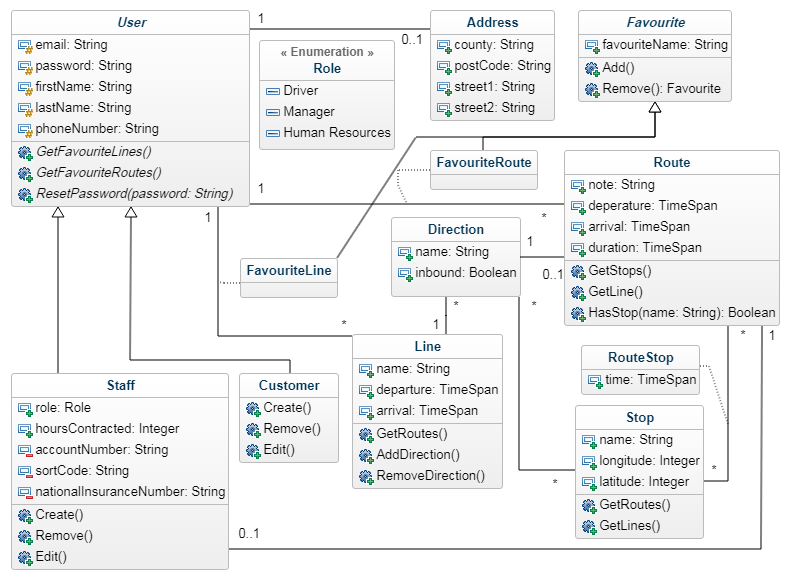
\includegraphics[width=\linewidth]{UMLClassDiagram}
    \caption{Initial class diagram, corresponding to what we thought
    the classes would look like based on the requirements analysis}
  \end{figure}

  \subsection{Final class diagram}
  \begin{figure}[ht]
    \centering
    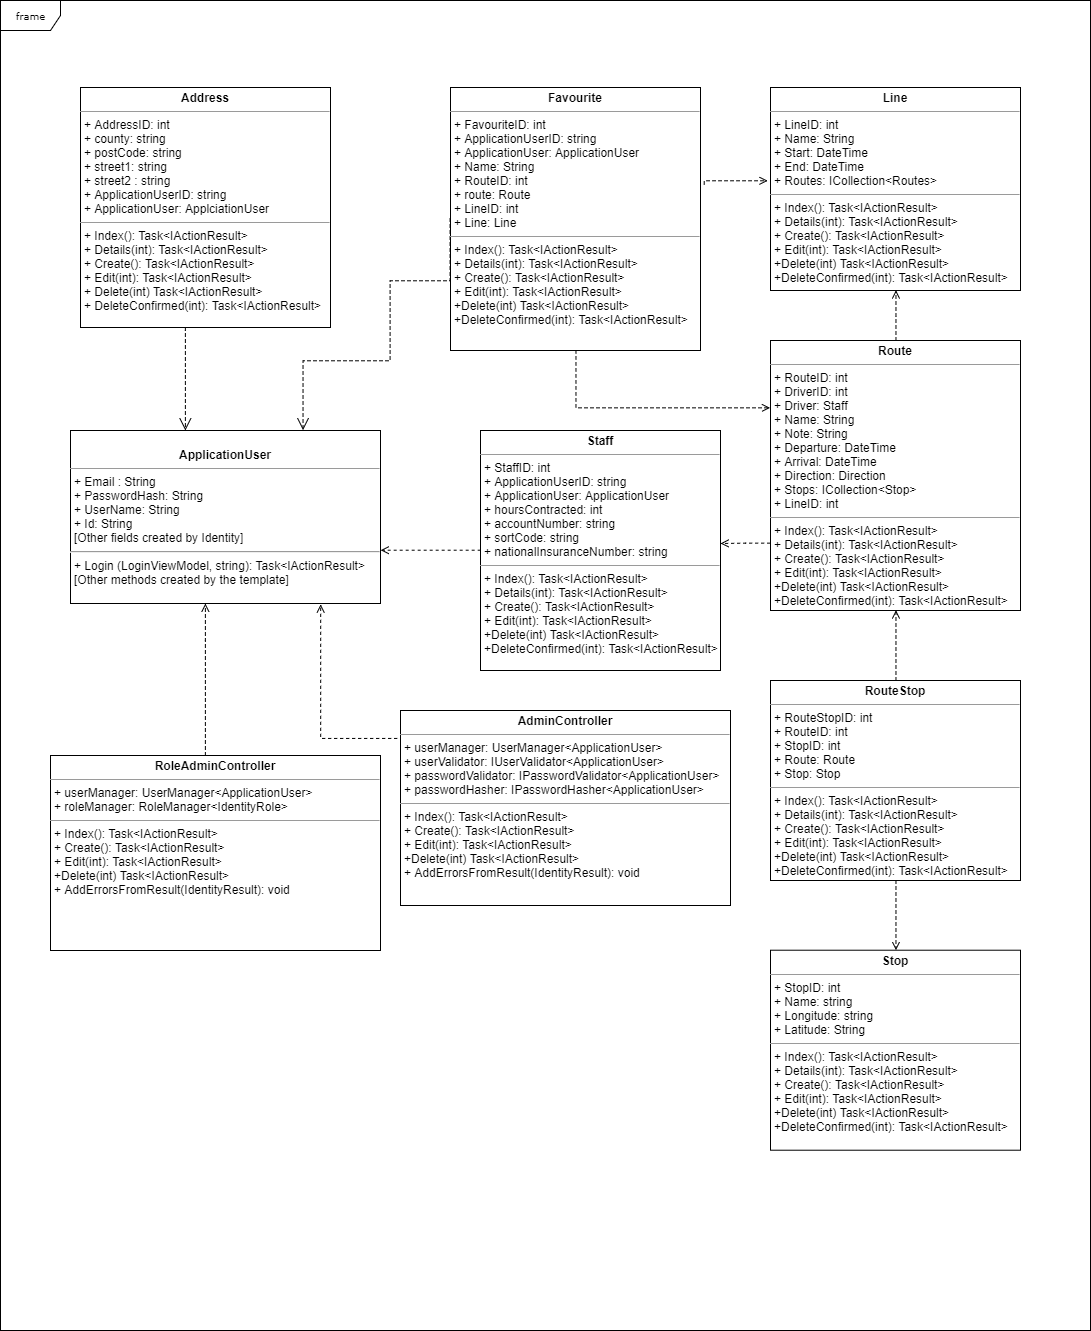
\includegraphics[width=\linewidth]{FinalClassDiagram}
    \caption{Final class diagram, obtained after scaffolding the
    views and developing the admin controllers}
  \end{figure}
  
  In order to obtain this diagram, we started by using the initial data previewed in the initial
  class diagram to create the models that would form our database. After that, we scaffolded the
  views and controllers, giving us the methods for the classes. The Admin and RoleAdmin controllers
  were custom developed from scratch in a series of trial and error until we managed to create
  the functionality that was necessary to us. The attributes that these two classes contain are
  just instances of classes and interfaces that allow to manipulate the users and roles tables
  in the database. In reality, that means that these controllers do not have any models associated
  nor entries in the database.